%%==========================================================================
%%==========================================================================
\section{Introduction}
La sécurité informatique est un axe important dans le monde de l'informatique. Ces dernières années, on peut constater que plusieurs méthodes de cryptographie ont été développées. Ces méthodes reposent sur les fonctions de hachage cryptographiques. Ce sont des fonctions qui associent à un message de longueur arbitraire une chaîne d'octets de longueur fixe appelée {\it{haché}}.\\

Les fonctions de hachage doivent satisfaire les principes suivant:
\begin{itemize}
  \item résistance au calcul de collision ;
  \item résistance au calcul de seconde pré-image ;
  \item résistance au calcul de pré-image.
\end{itemize}
\vspace{.5cm}

Une des fonctions de hachage les plus utilisées est MD5, inventée par Rivest en 1992. MD5 comme toute fonctions de hachage prend en entrée un message de longueur variable et retourne une chaîne de longueur fixe.\\

Le but de cette étude est de décrire le fonctionnement interne de la fonction de hachage MD5 et d'en réaliser un état de l'art sur sa résistance aux calcul de seconde pré-image à préfixe choisi.
Nous verrons ensuite quel(s) impact(s) une collision sur des certificats peut avoir en l'intégrant dans le transchiffrement.

%%==========================================================================
%%==========================================================================
\section{Le schéma de Merkle-Damgard}
Le schéma de Merkle-Damgard décrit comment construire une fonction de hachage à partir d'une fonction de compression. MD5 est basé sur ce schéma dont le principe de fonctionnement est le suivant:\\

\begin{figure}[h!]
  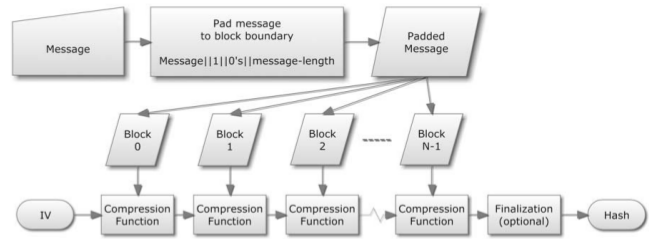
\includegraphics[scale=.61]{./images/md.png}
  \caption{Principe de fonctionnement de Merkle-Damgard}
\end{figure}

\vspace{.5cm}

\begin{itemize}
\item la fonction de compression prend en entrée un bloc B de taille 512 bits et une IHV (valeur de hachage intermédiaire) de 128 bits et rend un vecteur de 128 bits ;
\item chaque message passé en paramètre doit subir un padding si sa taille n'est pas multiple de 512 bits ;
\item le message est ensuite découpé en N blocs de 512 bits ;
\item la fonction de hachage commence avec une IHV initiale appelée {\it{IV}} ;
\item chaque bloc de message $M_{i}$ est appelé avec la valeur courante $IHV_{i}$ et la fonction de compression calcul une nouvelle valeur $IHV_{i+1}$. Lorsque tous les blocs sont traités le {\it{haché}} final $IHV_{N}$ est construit .
\end{itemize}
\vspace{.5cm}

%%==========================================================================
%%==========================================================================
\section{Fonctionnement de MD5}
MD5 fonctionne de la manière suivante:\\
\begin{enumerate}
\item {\it{\bf{le padding}}}. On ajoute un pad au message initial si sa longueur n'est pas un multiple de 512 bits. Le padding consiste à ajouter une séquence de bits dont le premier bit est à 1 suivi de 0 de telle sorte que la longueur résultante soit égale à 448 mod 512. Les bits restants sont utilisés pour ajouter la longueur du message initial ;
\item {\it{\bf{le partitionnement}}}. MD5 découpe le message original (avec un padding ou non) en N blocs $M_{1}$, ..., $M_{N}$ de 512 bits ;
\item {\it{\bf{le processus}}}. MD5 calcule des valeurs intermédiaires de haché, {\it{IHV}}.
  \begin{itemize}
  \item Chaque IHV est divisé en 4 mots de 32 bits (a, b, c, d).
  \item L'{\it{IV}} initiale est ($a_{0}$, $b_{0}$, $c_{0}$, $d_{0}$) = ($67452301_{16}$, $EFCDAB89_{16}$, $98BADCFE_{16}$, $10325476_{16}$).
  \item Chaque IHV est calculée en utilisant la fonction de compression MD5Compress telle que:\\ $IHV_{i}$ = MD5Compress($IHV_{i-1}$, $M_{i}$) ;
  \end{itemize}
\item {\it{\bf{le résultat}}}. Le {\it{haché}} produit est la concaténation en hexadécimal des dernières valeurs\\ (a, b, c, d) calculées.
\end{enumerate}

%%==========================================================================
%%==========================================================================
\section{La fonction de compression de MD5}
La fonction de compression de MD5 prend en paramètre une IHV de 128 bits et un bloc de message de 512 bits. Elle s'effectue en 64 étapes découpées en 16 tours. À chaque étape les opérations suivantes sont réalisées:\\

%%==========================================================================
\subsection{Les opérations internes}
\begin{enumerate}
\item {\bf{l'addition et sa constante AC}}:\\
$AC_{t}$ = 2\up{32}|sin(t + 1)| \hspace{.5cm} pour 0 <= t <= 64\\
AC est de longueur 32 bits.

\item \bf{la rotation gauche et ses constantes RC}:\\
($RC_{t}$, $RC_{t+1}$, $RC_{t+2}$, $RC_{t+3}$) =
$\left\{
\begin{array}{l}
  (7, 12, 17, 22)   \hspace{.8cm}pour \hspace{.2cm} t = 0, 4, 8, 12 \\
  (5, 9, 14, 20)  \hspace{1cm}pour \hspace{.2cm} t = 16, 20, 24, 28 \\
  (4, 11, 16, 23)  \hspace{.8cm}pour \hspace{.2cm} t = 32, 36, 40, 44 \\
  (6, 10, 15, 21)  \hspace{.8cm}pour \hspace{.2cm} t = 48, 52, 56, 60 \\
\end{array}
\right.$
\vspace{.5cm}
\item \bf{une fonction non-linéaire $f_{t}$}:\\

$f_{t}$(x, y, z) =
$\left\{
\begin{array}{l}
  F(x, y, z) = (x  \bigwedge y) \bigoplus (\bar x \bigwedge z) \hspace{1.128cm} 0 <= t < 16\\
  G(x, y, z) = (z  \bigwedge x) \bigoplus (\bar z \bigwedge y) \hspace{.97cm} 16 <= t < 32\\
  H(x, y, z) = x \bigoplus y \bigoplus z \hspace{2cm} 32 <= t < 48\\
  I(x, y, z) = y \bigoplus (x \bigvee \bar z) \hspace{2cm} 48 <= t < 64\\
\end{array}
\right.$
\vspace{.5cm}
\end{enumerate}

%%==========================================================================
\subsection{Traitement des blocs de message}
Les blocs de message sont découpés en 16 mots consécutifs $m_{0}$, ..., $m_{15}$. Les blocs de mots sont ensuite étendus à 64 mots $W_{t}$ pour 0 <= t < 64 de 32 bits chacun tels que:
\vspace{.5cm}

$W_{t}$ =
$\left\{
\begin{array}{l}
  m_{t} \hspace{2.8cm} 0 <= t < 16\\
  m_{(1 + 5t) mod 16} \hspace{1cm} 16 <= t < 32\\
  m_{(5 + 3t) mod 16} \hspace{1cm} 32 <= t < 48\\
  m_{(7t) mod 16} \hspace{1.4cm} 48 <= t < 64\\
\end{array}
\right.$
\vspace{.5cm}

%%==========================================================================
\subsection{État interne de la fonction de compression}
Lors de chaque appel de la fonction de compression de MD5, son état interne est sauvegardé. L'état interne n'est autre que les mots $m_{t}$ vus dans la section précédente. Chaque mot est sauvegardé dans un registre Q = {$Q_{t}$, $Q_{t-1}$, $Q_{t-2}$, $Q_{t-3}$}. Le nouvel état $Q_{t+1}$ est calculé en initialisant ($Q_{t}$, $Q_{t-1}$, $Q_{t-2}$, $Q_{t-3}$) = (b, c, d, a) pour {\it{t}} = 0, 1, ..., 63, $Q_{t}$ est calculé comme suit:
\vspace{.5cm}

$\left\{
\begin{array}{l}
  F_t = f_t(Q_t, Q_{t-1}, Q_{t-2}) \\
  T_t = F_t + Q_{t-3} + AC_t + W_t \\
  R_t = RL(T_t, RC_t) \\
  Q_{t+1} = Q_t + R_t \\
\end{array}
\right.$
\vspace{.5cm}

Lorsque toutes les étapes de calcul sont finies l'état des mots finaux est ajouté à l'IHV et la fonction retourne comme valeur MD5Compress(IHV, B) = (a + $Q_{61}$, b + $Q_{64}$, c + $Q_{63}$, d + $Q_{62}$).

%%==========================================================================
\subsection{L'algorithme de fonction de compression}
L'algorithme de fonction de collision est réalisé de la manière suivante:\\

\begin{algorithm}
\caption{Algorithme de la fonction de compression}
\begin{algorithmic} 
\REQUIRE $m_0 ... m_{15} \hspace{.2cm} et \hspace{.2cm} (Q_{-3}, Q_{-2}, Q_{-1}, Q_0) = IV $\\
{\bf{for}} i = 0 .. 63 {\bf{do}}\\
\hspace{.5cm}$Q_{i+1} = Q_i +  (f_i(Q_i, Q_{i-1}, Q_{i-2}) + Q_{i-3} + AC_i + W_i) <<< S_i$\\
{\bf{end}}\\
{\bf{return}} $(Q_61 + Q_{-3}, Q_62 + Q_{-2}, Q_63 + Q_{-1}, Q_64 + Q_0)$
\end{algorithmic}
\end{algorithm}


%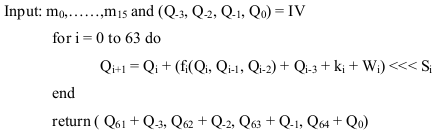
\includegraphics[scale=.61]{./images/algocom.png}

%%==========================================================================
\subsection{Schématisation du fonctionnement de MD5}
La fonction de MD5 est montrée par le schéma suivant, où $CV_{q}$ est l'ensemble des chaînes IHV, $Y_{q}$ est le q\up{ième} bloc de message de longueur 512 bits.\\

\begin{figure}[h!]
  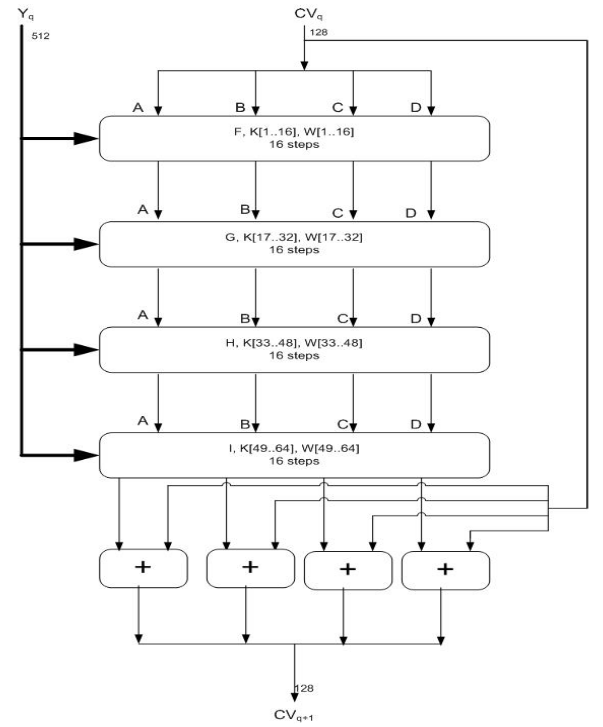
\includegraphics[scale=.61]{./images/md5process.png}
  \caption{Fonctionnement de MD5}
\end{figure}


%%==========================================================================
%%==========================================================================
\section{Étude de failles sur MD5}

Les premières collisions ont été trouvées par les équipes de Wang et Yu en 2004.  Leur procédé s'appuie sur la cryptanalyse de la fonction de compression de la fonction de hachage de MD5. 

Leur technique consistait à trouver des collisions en exécutant une seule fois la fonction de compression MD5 en analysant les changements effectués sur les bits à chaque tours.

%%==========================================================================
\subsection{Présentation de l'attaque menée par Wang et Yu}
L'attaque proposée par Wang et Yu est une attaque par collision. Le but est de trouvé deux message différents M et M' qui ont le même haché MD5.\\

L'intérêt de cette attaque est de calculer deux blocs de collisions. Le premier bloc (resp. le second bloc) dépend des premiers blocs du message (resp. des seconds blocs) des messages M et M'. On a alors les messages M et M' qui se découpent ainsi:
\begin{itemize}
  \item M = ($M_{0}$, $M_{1}$)
  \item M' = ($M'_{0}$, $M'_{1}$)
\end{itemize}
où chaque $M_{i}$ et $M'_{i}$ est un bloc de 512 bits ayant chacun 16 mots de 32 bits.\\

Wang a appliqué la fonction MD5 identiques au premiers bloc des messages M et M' et obtenu deux haché différents h et h'. Les vecteurs initiaux lors de l'appel de la fonction MD5  sur les premiers blocs de M et M' sont identique. h1 et h2 sont sauvegardés puis réutilisé pour calculer le second bloc de collision à l'aide des seconds blocs de message de M et M'. Le haché produit par la fonction de hachage sur les seconds blocs de messages M et M' devra être identique. Ce qui se traduit de la manière qui suit:\\

\begin{itemize}
\item (a, b, c, d) = MD5($a_0, b_0, c_0, d_0, M_0$)
\item (a', b', c', d') = MD5($a_0, b_0, c_0, d_0, M'_0$)
\item on a MD5($a, b, c, d, M_1$) = MD5($a', b', c', d', M'_1$).
\end{itemize}

où $a_0, b_0, c_0, d_0$ désignent les valeurs initiales de la fonctions MD5.\\

Pour parvenir au résultat précédent, Wang utilise une attaque dite différentielle.


\subsubsection{Attaque différentielle sur MD5 menée par Wang et Yu}
L'attaque différentielle menée par wang sur deux messages M = ($M_0, M_1$) et M' = ($M'_0, M'_1)$) d'une longueur l-bits est construit comme suit: 
$\Delta$$H_0$ -->\up{$M_0, M'_0$} $\Delta$$M_1$ -->\up{$M_1, M'_1$} --> $\Delta$$H$.\\

On considère que pour le message M, l'IV initial de MD5 est IV = (a, b, c, d) et que le vecteur du second bloc est $IV_{1}$ = ($a_{1}$, $b_{1}$, $c_{1}$, $d_{1}$) = ($Q_{61}$, $Q_{64}$, $Q_{63}$, $Q_{62}$) + (a, b, c, d) et où ($Q_{61}$, $Q_{64}$, $Q_{63}$, $Q_{62}$) = $MD5_{1..64}$(IV, $M_{0}$) et la valeur haché h est h = $MD5_{1..64}$($IV_{1}$, $M_{1}$) + ($a_{1}$, $b_{1}$, $c_{1}$, $d_{1}$). De la même manière on va définir les valeurs $IV'_{1}$ et h' pour les messages $M'_{0}$ et $M'_{1}$ de M'.\\

La différence modulaire passée en entrée de la fonction MD5 doit respecter les conditions suivantes:
\begin{itemize}
\item $\Delta$$M_{0}$ = $M'_{0}$ - $M_{0}$ = (0, 0, 0, 0, 2\up{31}, 0, 0, 0, 0, 0, 0, 2\up{15}, 0, 0, 2\up{31}, 0)
\item $\Delta$$M_{1}$ = $M'_{1}$ - $M_{1}$ = (0, 0, 0, 0, 2\up{31}, 0, 0, 0, 0, 0, 0, -2\up{15}, 0, 0, 2\up{31}, 0)
\item $\Delta$$IV_{1}$ = $IV'_{1}$ - $IV_{1}$ = (2\up{31}, 2\up{25} + 2\up{31}, 2\up{25} + 2\up{31},2\up{25} + 2\up{31})
\item $\Delta$h = h' - h = (0, 0, 0, 0)
\end{itemize}
\vspace{.5cm}

Cette méthode permet de trouver des blocs de collisions en deux itérations ou les messages qui ont été trouvés pour effectuer les collisions sont constitués de deux blocs de collisions d'une longueur totales de 1024 bits.

Grâce à la différence effectuée entre les premiers et seconds blocs des messages, il est possible de trouver les différences qui existent entre les bits de chaque bloc.

En calculant la différence entre les bits de chaque bloc de collision, il est alors possible de donner un ensemble de bits de conditions qui assurent la différence entre les bits des blocs un et deux de chaque message.



\subsubsection{Algorithme de l'attaque menée par Wang et Yu}
\begin{enumerate}
\item Répéter les étapes suivantes jusqu'à trouver le premier bloc de collision.
  \begin{itemize}
  \item (a) selectionner un message aléatoire $M_0$ ;
  \item (b) modifier $M_0$ de fa\c con à respecter les bits de conditions
  \item (c) les conditions respectées, les premiers blocs $M_0 et M'_0$ produisent les premières différences de blocs qui seront utilisées pour calculer le second bloc de collision.
  \end{itemize}
\item Répéter les étapes suivantes jusqu'à ce qu'une collision soit trouvée.
 \begin{itemize}
 \item (a) choisir aléatoirement un message $M_1$
 \item (b) modifier $M_1$ pour satisfaire les bits de conditions
 \item (c) si les conditions sont respectées la différence entre les IHV doit être nulle.
 \end{itemize}
\end{enumerate}


$\Delta$$H_0$ désigne la différence initiale entre les valeurs initiales IV et IV'. $\Delta$H est la différence en sortie des deux messages. Si $\Delta$H = 0, alors il y'a une collision entre M et M'.

%%==========================================================================
\subsection{Présentation de l'attaque menée par Marc Stevens}
Marc Stevens reprend les travaux réalisés par Wang et Yu et améliore leurs algorithmes en y introduisant de nouvelles notions et montre comment à partir de deux messages arbitraires, il est possible de générer des collisions sous MD5.\\

La différence technique entre ces deux travaux repose sur le fait que pour créer une collision, Stevens utilise un seul bloc de collision au lieu de deux comme le faisait Wang et Yu. 

\subsubsection{Attaque à préfixes choisis}
Contrairement à la méthode utilisée par Wang et Yu, les deux messages initiaux peuvent avoir des longueurs différentes. Dans ce cas, il faut appliquer un padding au plus court des deux, pour que les messages aient des longueurs égales. Quand les messages seront passés à la fonction de compression de MD5, ils auront donc le même padding.

L'idée principale est d'éliminer la différence $\Delta$IHV en r étapes où r désigne les étapes pour construire r bloc de quasi collisions.

\subsection{Algorithme de la méthode de Marc Stevens}
\begin{figure}[h!]
  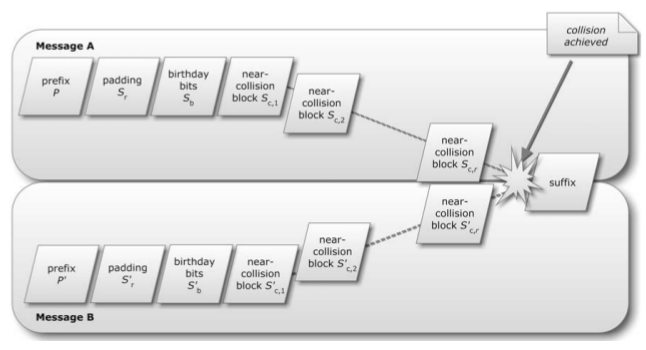
\includegraphics[scale=.61]{./images/col.png}
  \caption{Algorithme de recherche des blocs de quasi-collisions}
\end{figure}


\subsubsection{Construction des préfixes choisis de collisions}
Un préfixe choisi de collision est un couple de messages (M, M') qui consiste à choisir arbitrairement des préfixes P et P', construire avec des suffixes S et S' de telle sorte que l'on ait:\\
M = P || S et M' = P' || S' et MD5(M) = MD5(M').\\


Les suffixes S et S' ont la même structure. Ils sont découpés en 3 parties.
\begin{itemize}
\item le "padding" $S_{r}$. $S_{r}$ est choisi tel que P || $S_{r}$ || $S_{b}$ ou P' || $S'_{r}$ || $S'_{b}$ soit multiple de 512 ;
\item les bits d'anniversaire $S_{b}$. Ils sont choisis de façon à respecter une certaine condition (chemin différentiel) et servent à réduire le nombre d'appel de la fonction de compression de MD5 pour parvenir à trouver une collision. En introduisant cette chaîne de bits on parvient ainsi d'un nombre d'appel de 2\up{59} à 2\up{39}. Ce qui reste largement en dessous du temps limite de calcul que l'on peut faire de nos jours ;
\item bit de quasi-collision $S_{c}$. Utilisé pour éliminer la différence (delta) $IHV_N$ = $IHV_N$ - $IHV'_N$ où $IHV_N$ (resp. $IHV'_N$) est le résultat IHV renvoyé par la fonction MD5Compress appliquée au message P || $S_{r}$ || $S_{b} || S_c$ (resp. P' || $S'_{r}$ || $S'_{b} || S'_c$) .
\end{itemize}
\vspace{.5cm}


\subsubsection{Chemin différentiel et bits de conditions}
Nous avons vu avant l'état interne lors d'un appel de la fonction de compression de MD5. Si on applique MD5Compress aux entrées (IHV, B) et (IHV', B') le chemin différentiel de la fonction MD5Compress est défini de la fa\c con suivante.\\

$\left\{
\begin{array}{l}
  \Delta F_t = f_t(Q'_t, Q'_{t-1}, Q'_{t-2}) - f_t(Q_t, Q_{t-1}, Q_{t-2}) \\
  \Delta T_t = \Delta F_t + \Delta Q_{t-3} + \Delta W_t \\
  \Delta R_t = RL(T'_t, RC_t) - RL(T_t, RC_t) \\
  \Delta Q_{t+1} = \Delta Q_t + \Delta R_t \\
\end{array}
\right.$
\vspace{.5cm}

La propagation du chemin différentiel se fait à travers les 64 étapes de la fonction MD5 . Le chemin différentiel est calculé à partir de $\Delta$IHV et $\Delta$B.

\subsubsection{Les bits de conditions}
Le chemin différentiel est calculé à l'aide de bits de conditions à un état t du mot sauvegardé par la fonction de compression de MD5. En d'autres termes, le chemin différentiel est calculé sur $Q_t$ et $Q'_t$ où un bit de condition peut être calculé de manière directe ou indirecte à partir des valeurs de bits de $Q_t$[i] et $Q'_t$[i]. Le chemin différentiel est alors une matrice de 68 lignes (-3 <= t <= 64) et 32 colonnes pour chaque bit.\\

Un bit de condition direct sur un état Q ou Q' ne doit pas modifier d'autres bits de cet état Q où Q'. Un bit de condition direct par contre peut modifier l'état d'un bit de Q ou Q'. Les bits de conditions sont donnés comme suit:\\


\begin{tabular}{lll}
\hline
	$Q_t$[i] &\vline \hspace{.1cm} Condition sur ($Q_t$[i], $Q'_t$[i]) &\vline \hspace{.1cm} $k_i$ \\ \hline
	. &\vline \hspace{.1cm} $Q_t$[i] = $Q'_t$[i] &\vline \hspace{.1cm} 0 \\ \hline
	+ &\vline \hspace{.1cm} $Q_t$[i] = 0, $Q'_t$[i] = 1 &\vline \hspace{.1cm} +1 \\ \hline
	- &\vline \hspace{.1cm} $Q_t$[i] = 1, $Q'_t$[i] = 0 &\vline \hspace{.1cm} -1 \\ \hline
\end{tabular}

\subsubsection{Construction du chemin différentiel}
la construction du chemin différentiel est définie par l'algorithme suivant: 
\begin{itemize}
  \item Utiliser IHV et IHV' qui détermine les bits de conditions ($Q_i$) -3 <= i <= 0
  \item Construire un chemin différentiel partiel dit faible pour les étapes 0 ... 11 de la fonction de hachage MD5 en étendant les $q_i$.
  \item La construction d'un chemin différentiel partiel dit fort pour les étapes 16 ... 63 de la fonction de hachage MD5 en étendant les $q_i$.
    \item essayer de connecter les deux chemins différentiels aux étapes 12 ... 15. Si ce n'est pas possible, rechercher d'autres chemins différentiels dit fort et faible qui remplissent les conditions.
\end{itemize}

%%==========================================================================
\subsection{Complexité des attaques sur MD5}

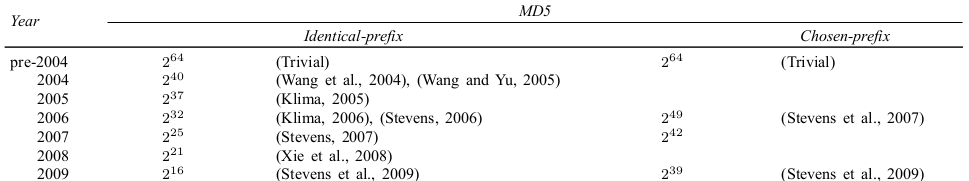
\includegraphics[scale=.50]{./images/complexite.png}

\vspace{.5cm}
Au cours du temps les méthodes de cryptanalyse utilisant les résultats des recherches de Wang et Yu sur MD5 ont été améliorées. 

L'algorithme proposé par Wang en 2004 nécessite environ 2\up{39} opérations pour la recherche du premier bloc et 2\up{32} opérations pour la recherche du second bloc.

L'algorithme proposé par Marc Stevens en 2012 peut nécessiter moins de 2\up{30} opérations pour trouver un bloc de collision.

%%==========================================================================
%%==========================================================================
\section{Application d'exploitation de collision MD5}

L'état de l'art de la collision MD5 faite dans les chapitres précédents peut être appliqué dans la vie réelle. On peut citer par exemple, la collision entre documents, la vérification de l'intégrité d'un logiciel ou encore, en ce qui nous concerne, la création de faux certificats d'autorité. \\

Dans ce chapitre, nous allons voir comment construire deux certificats X.509 avec des noms distinctifs mais ayant la même signature électronique.



%%==========================================================================
\subsection{Rappel sur les certificats X.509}

X.509 est une norme de cryptographie de l'union internationale des télécommunications pour les infrastructures à clés publiques (PKI). Il établit entre autres les formats standards de certificats électroniques et un algorithme pour la validation de chemin de certification. X.509 à été créé en 1988  et repose sur un système hiérarchique d'autorités de certification, à l'inverse des réseaux de confiance (comme PGP), où n'importe qui peut signer (et donc valider) les certificats des autres.\\

Dans le système X.509, une autorité de certification attribue un certificat liant une clé publique à un nom distinctif (Distinguish Name), à une adresse électronique ou un enregistrement DNS.\\

Les certificats racines sont des clés publiques non signées, ou auto-signées, dans lesquels repose la confiance. Des autorités de certification commerciales détiennent des certificats racines présents dans de nombreux logiciels, par exemple les navigateurs Web. Quand le navigateur ouvre une connexion sécurisée (SSL) vers un site ayant acheté une certification auprès d'une autorité connue, il considère le site comme sûr dans la mesure où le chemin de certification est validé. Le passage en mode sécurisé est alors transparent.\\

Si le certificat est auto-signé (autorité de certification et créateur de la clé publique ne font qu'un), le navigateur propose de l'examiner, puis de l'accepter ou de le refuser selon la confiance qu'on lui accorde.\\

%%==========================================================================
\subsection{Structure d'un certificat}

\begin{minipage}{.4\linewidth}
\begin{itemize}
\item Version
\item Numéro de série
\item Algorithme de signature du certificat
\item Nom du signataire du certificat
\item Validité (dates limite) 
  \begin{itemize} 
  \item Pas avant
  \item Pas après
  \end{itemize}
\item Détenteur du certificat
\item Informations sur la clé publique :
  \begin{itemize}
  \item Algorithme de la clé publique
  \item Clé publique proprement dite
  \end{itemize}
\item Identifiant unique du signataire (optionnel, à partir de X.509 version 2)
\item Identifiant unique du détenteur du certificat (optionnel, à partir de X.509 version 2)
\item Extensions (optionnel, à partir de X.509 version 3)
  \begin{itemize}
  \item Liste des extensions
  \end{itemize}
\end{itemize}
\end{minipage}\hfill
\begin{minipage}{.4\linewidth}
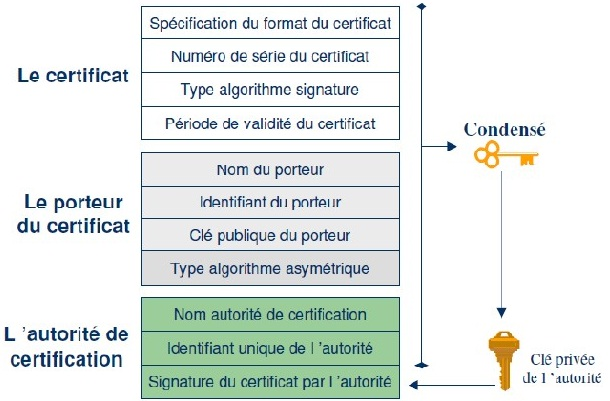
\includegraphics[width=8cm, height=7cm]{./images/cert.jpg}
\end{minipage}


%%==========================================================================
\subsection{Création d'un faux certificat}
Lorsque l'on génère deux certificats X.509 qui ont des signatures identiques mais des Distinguish Name différents on intervient directement sur le module RSA (la clé publique).\\

Nous avons vu que pour générer une collision à préfixe choisi, il faut calculer des préfixes qui permettent de calculer des collisions. En application sur les certificats, le préfixe du vrai certificat contient le DN (distinguish name) ainsi que les 208 premiers bits du module RSA.

Le préfixe du faux certificat contient le nom de la fausse autorité, une clé publique RSA de 1024 bits et la première partie des champs d'extension du certificat. Le champ d'extension rempli est "basic constraint" qui contient un bit qui identifie le certificat comme une autorité en mettant la variable CA à TRUE.\\

Ces deux préfixes de collisions construits, les bits de collisions sont calculés à l'aide des bits d'anniversaire et des blocs de quasi collision.

\subsection{Modification des bits d'un certificat}
Les bits d'anniversaire introduits pour calculer les blocs de collisions sont au nombre de 96 et directement situés après, on y trouve les blocs d'entrée de la fonction MD5.

Après les bits d'anniversaire, on trouve les blocs de quasi collision de 512 bits chacun. Sur le vrai certificat, cela se résume à 208 + 96 + x * 512 = p bits du module RSA, où x est le nombre de bloc de quasi collision. Prenons comme exemple x = 3, on a alors 208 + 96 + 3 * 512 = 1840 bits.

On sait que la longueur du module RSA est de 2048 bits. On constate qu'on a alors 2048 - 1840 = 208 bits après les bits de collisions qu'ils reste pour compléter les 2048 bits du module RSA du vrai certificat. Ces 208 bits doivent être déterminés de telle sorte que la factorisation du module RSA soit connue.

%%==========================================================================
\subsection{Détails de construction des certificats}
\begin{enumerate}
\item Il faut créer deux certificats de telle sorte que tous les champs soit remplis excepté, le module de la clé publique RSA et la signature. En s'assurant que:
 \begin{itemize} 
 \item les données doivent être de la forme X.509 ;
 \item la longueur d'octets du module et de l'exposant publique doivent être fixé ;
 \item contrôler la position où commence la partie du module RSA en rajoutant des informations au Distinguish Name ;
\end{itemize}
\item appliquer MD5 sur les champs des parties à être signer des certificats de façon à obtenir des IHVs que l'on utilisera pour l'étape qui suit ;
\item On utilise les IHVs et leur blocs correspondants en y ajoutant les bits d'anniversaires plus précisément 96 bits, ce qui équivaut à la satisfaction des 96 bits de différence entre les IHVs en sortie.
\item Il faut calculer la différence de chaîne d'octets entre les blocs proches de collision $S_{c}$ et $S'_{c}$ de 4096 bits chacun. Comme vu précédement, chaque bloc de quasi-collision est utilisé pour éliminé la différence entre les IHVs de l'étape précédente de telle sorte que la différence entre les IHVs soit nulle. À ce stade une collision MD5 à été accomplie. S = $S_{b}$ || $S_{c}$ et S' = $S'_{b}$ || $S'_{c}$ sont alors de longueur 4192 bits sur le module RSA ;
\item on construit le module RSA sécurisé de 8192 bits, des chaîne d'octets S et S' de longueur 4192 bits chacune en y ajoutant une chaîne identique de 4000 bits ;
\item on complète le premier certificat en y insérant les informations de la clé publique. On calcule ensuite le haché MD5 de "la partie à être signée" et on l'utilise pour calculer la signature que l'on ajoutera au premier certificat et ainsi finir sa construction ;
\item ajouter les informations de la clé publique et la même signature dans le second certificat pour compléter sa construction.	
\end{enumerate}
\vspace{.5cm}

Comme on peut le voir, les étapes 3 et 4 sont primordiales mais également les plus difficiles.


\section{Difficultés rencontrées}
Au cours de cette étude, nous nous sommes heurtés à quelques difficultés. Tout d'abord la recherche d'éléments pouvant nous conduire à l'élaboration d'un algorithme permettant la construction d'une collision sur des certificats. En effet la plupart des documents ont été soit sciemment enlevés de toute publication, soit certains détails primordiaux ont été volontairement supprimés. Ceci s'explique par le fait que la découverte de Wang et Yu à été utilisée à des fins non morales.

En second lieu vient la compréhension des bits de conditions et la génération du chemin différentiel dans la recherche des préfixes de collision. Pour cela il faut bien comprendre comment marche la cryptanalyse de la fonction de hachage MD5 en particulier de la fonction de compression MD5Compress et de ses opérations internes.

\newpage
%%==========================================================================
%%==========================================================================
